\section{Результаты измерений}
\newcommand{\lissaju}[1]{\begin{figure}[ht!]\centering\includegraphics[width=0.8\linewidth]{img/#1}\caption{Отношение частот: #1}\end{figure}}

\lissaju{1:1}
\lissaju{2:1}
\lissaju{3:1}
\lissaju{3:2}
\lissaju{4:3}
\lissaju{5:2}

\begin{figure}[ht!]\centering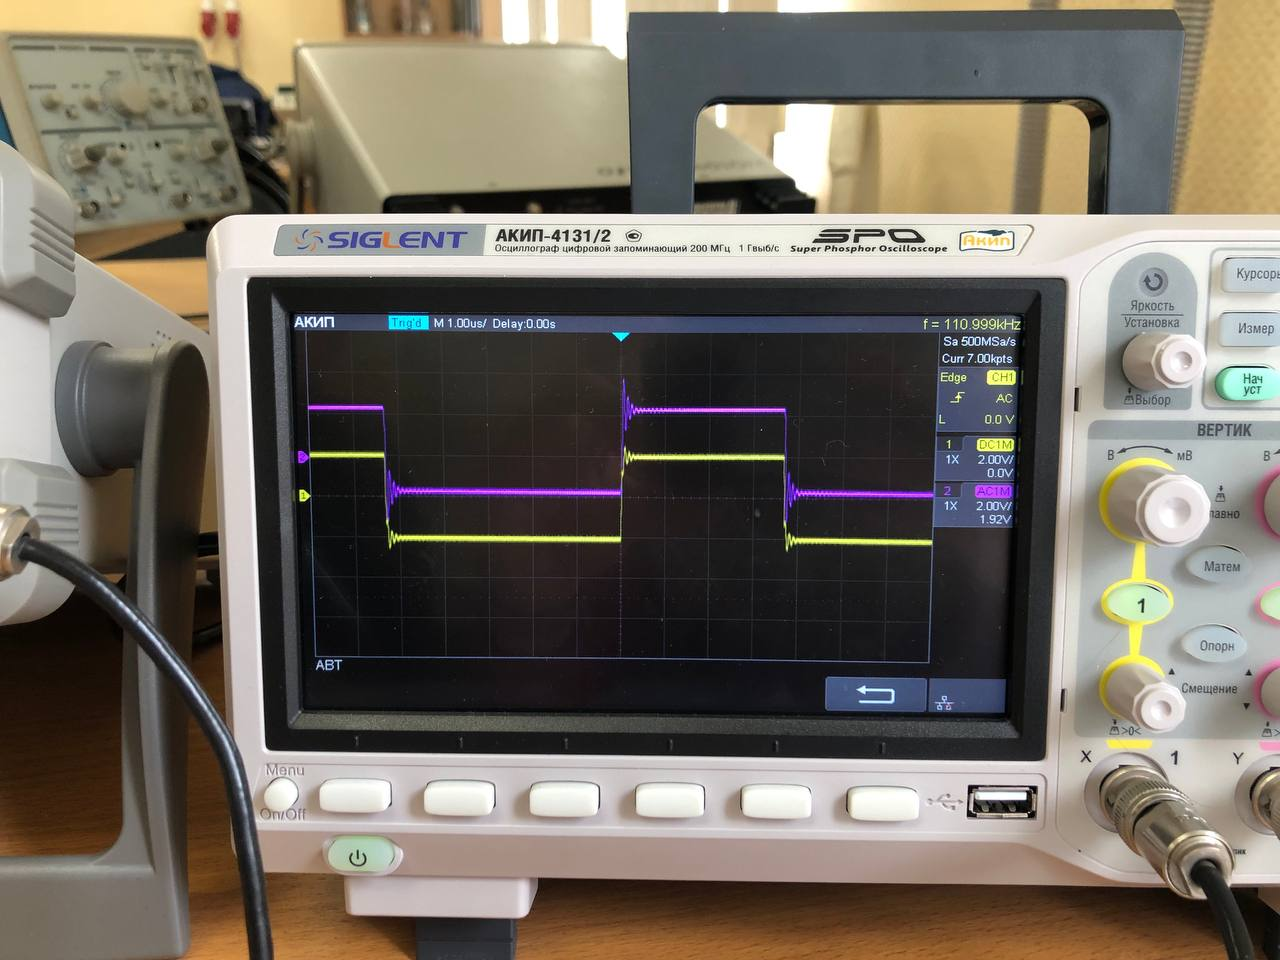
\includegraphics[width=0.8\linewidth]{img/shit1}\end{figure}
\begin{figure}[ht!]\centering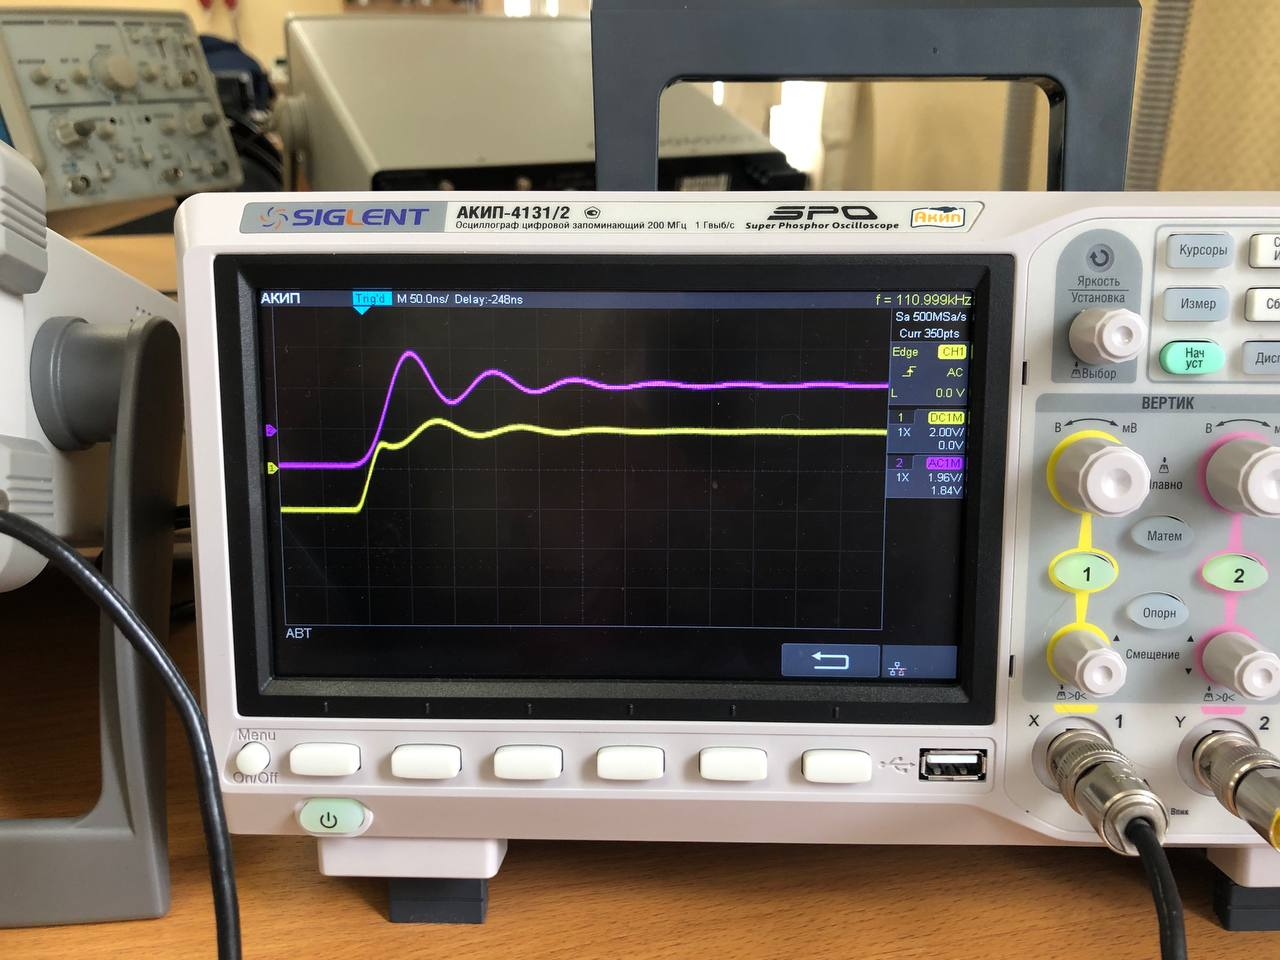
\includegraphics[width=0.8\linewidth]{img/shit2}\end{figure}

\begin{table}[ht!]
    \caption{Измерения частоты аналоговым осциллографом}
    \begin{tabular}{|l|l|l|l|l|l|l|l|}
    \hline
    $\nu_0,\,\text{Гц}$ & $T,\,\text{дел}$ & TIME/DIV, мс & $T,\,\text{мс}$ & $\nu,\,\text{Гц}$ & $\delta T,\,\text{мс}$ & $\delta\nu,\,\text{Гц}$ & $\nu - \nu_0,\,\text{Гц}$ \\ \hline
    $1000$              & $1$              & $1$          & $1$             & $1000$            & $0{,}1$                & $100$                   & $0$                       \\ \hline
    $800$               & $1{,}2$          & $1$          & $1{,}2$         & $833$             & $0{,}1$                & $69$                    & $33$                      \\ \hline
    $600$               & $1{,}8$          & $1$          & $1{,}8$         & $556$             & $0{,}1$                & $31$                    & $-44$                     \\ \hline
    $400$               & $2{,}4$          & $1$          & $2{,}4$         & $417$             & $0{,}1$                & $17$                    & $17$                      \\ \hline
    $200$               & $5$              & $1$          & $5$             & $200$             & $0{,}1$                & $4$                     & $0$                       \\ \hline
    \end{tabular}
\end{table}

Присоединим генератор к аналоговому осциллографу и измерим частоту сигнала, потом то же
самое сделаем с цифровым.

\begin{table}[ht!]
    \caption{Изсмерения цифровым осциллографом (курсорами~--- величины с индексом 1, 
    без них~--- с индексом 2)}
    \begin{tabular}{|l|l|l|l|l|l|l|l|l|}
    \hline
    $\nu_0,\,\text{Гц}$ & $T_1,\,\text{мс}$ & $T_2,\,\text{мс}$ & $\delta T_1,\,\text{мс}$ & $\delta T_2,\,\text{мс}$ & $\nu_1,\,\text{Гц}$ & $\nu_2,\,\text{Гц}$ & $\delta\nu_1,\,\text{Гц}$ & $\delta\nu_2,\,\text{Гц}$ \\ \hline
    $1000$              & $1$               & $1$               & $0{,}01$                 & $0{,}00005$              & $1000$              & $1000$              & $0{,}01$                  & $0{,}00005$               \\ \hline
    $800$               & $1{,}25$          & $1{,}25$          & $0{,}01$                 & $0{,}0000625$            & $800$               & $800$               & $0{,}008$                 & $0{,}00005$               \\ \hline
    $600$               & $1{,}67$          & $1{,}67$          & $0{,}01$                 & $0{,}0000833$            & $600$               & $600$               & $0{,}006$                 & $0{,}00005$               \\ \hline
    $400$               & $2{,}5$           & $2{,}5$           & $0{,}01$                 & $0{,}000125$             & $400$               & $400$               & $0{,}004$                 & $0{,}00005$               \\ \hline
    $200$               & $5$               & $5$               & $0{,}1$                  & $0{,}00025$              & $200$               & $200$               & $0{,}02$                  & $0{,}00005$               \\ \hline
    \end{tabular}
\end{table}

Измерим максимальную и минимальную амплитуды при $\nu_0=1000\,\text{Гц}$.
$U_{max}=20\pm 1\,\text{В}$, $U_{min}=4\pm 1\,\text{мВ}$.

\begin{table}[!ht]
    \centering
    \caption{Измерение АЧХ цифрового осциллографа}
    \begin{tabular}{|l|l|}
    \hline
        $\nu,\,\text{кГц}$ & $U,\text{В}$ \\ \hline
        30000 & 5 \\ \hline
        300 & 5.2 \\ \hline
        30 & 5.2 \\ \hline
        3 & 5.2 \\ \hline
        0.003 & 5.2 \\ \hline
        3000 & 5.2 \\ \hline
        10000 & 5.2 \\ \hline
        20000 & 5 \\ \hline
        15000 & 5.08 \\ \hline
        11000 & 5.16 \\ \hline
        12000 & 5.16 \\ \hline
        13000 & 5.12 \\ \hline
        14000 & 5.12 \\ \hline
        16000 & 5.08 \\ \hline
        17000 & 5.04 \\ \hline
        18000 & 5.04 \\ \hline
        19000 & 5.04 \\ \hline
    \end{tabular}
\end{table}

\begin{figure}[ht!]\centering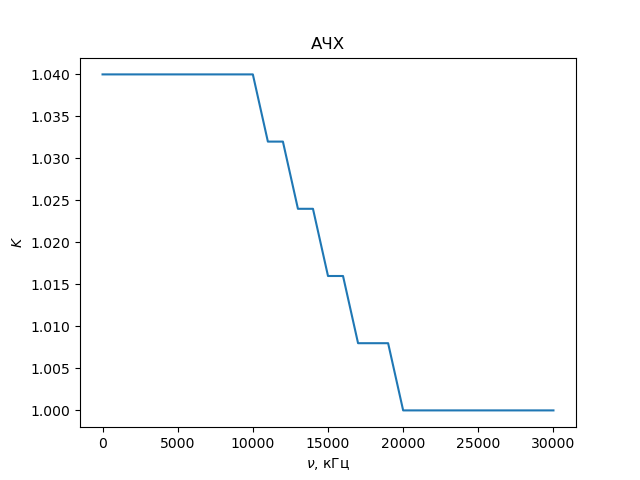
\includegraphics[width=0.8\linewidth]{img/ach}\end{figure}

Прямоугольные импульсы можно представить в виде суперпозиции бесконечного числа
гармонических колебаний с разными частотами. Часть из этих частот очень велика и
искажается АЧХ осциллографа, поэтому сигнал на границах ступенек осциллирует.

При частотах от $8$ до $20\,\text{МГц}$ прямая переходит в эллипс, а потом
в горизонтальную прямую. 

\begin{table}[ht!]
    \caption{Изучение сдвига фаз}
    \begin{tabular}{|l|l|l|l|l|l|}
    \hline
    $\nu,\,\text{МГц}$ & $y_0,\,\text{Мв}$ & $A_y,\,\text{В}$ & $\sin\Delta\phi$ & $\Delta\phi$ & $\lg\nu$  \\ \hline
    $14$              & $448{,}9$         & $2{,}881$        & $0{,}156$        & $2{,}985$    & $7{,}146$ \\ \hline
    $15$              & $777{,}2$         & $2{,}439$        & $0{,}319$        & $2{,}817$    & $7{,}176$ \\ \hline
    $16$              & $522{,}6$         & $1{,}782$        & $0{,}293$        & $2{,}844$    & $7{,}204$ \\ \hline
    $13$              & $1394$            & $4{,}663$        & $0{,}299$        & $2{,}838$    & $7{,}114$ \\ \hline
    $12$              & $1{,}96$          & $7{,}37$         & $0{,}0002$       & $3{,}141$    & $7{,}079$ \\ \hline
    \end{tabular}
\end{table}
\begin{figure}[ht!]\centering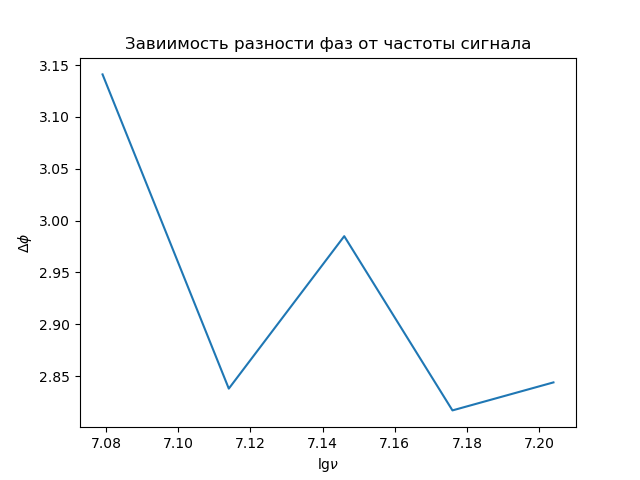
\includegraphics[width=0.8\linewidth]{img/kek}\end{figure}

В интервале от $8$ до $20\,\text{МГц}$ нельзя проводить измерения из-за большой
разнотсти фаз.

\newpage
~
\newpage
~
\newpage
~
\newpage
~
\newpage
~
\newpage
~

\section{Вывод}

Я изучил устройство цифрового и электронного осциллографа и научился изучать периодические
процессы с их помощью.
